\section{Testing}
\indent\indent We have a model based on the simulated annealing algorithm, which is influenced by various parameters such as the maximum value of parameter variation (strides) and initial and final temperatures. We will conduct stability tests on these two parameters to evaluate the stability of the model.\\
\indent First, we keep the initial and final temperatures and parameter values unchanged in the algorithm. We adjust the strides to be 0.3 and 0.6, respectively, and run the program. The final results are as follows:
\begin{figure}[H]
    \centering
    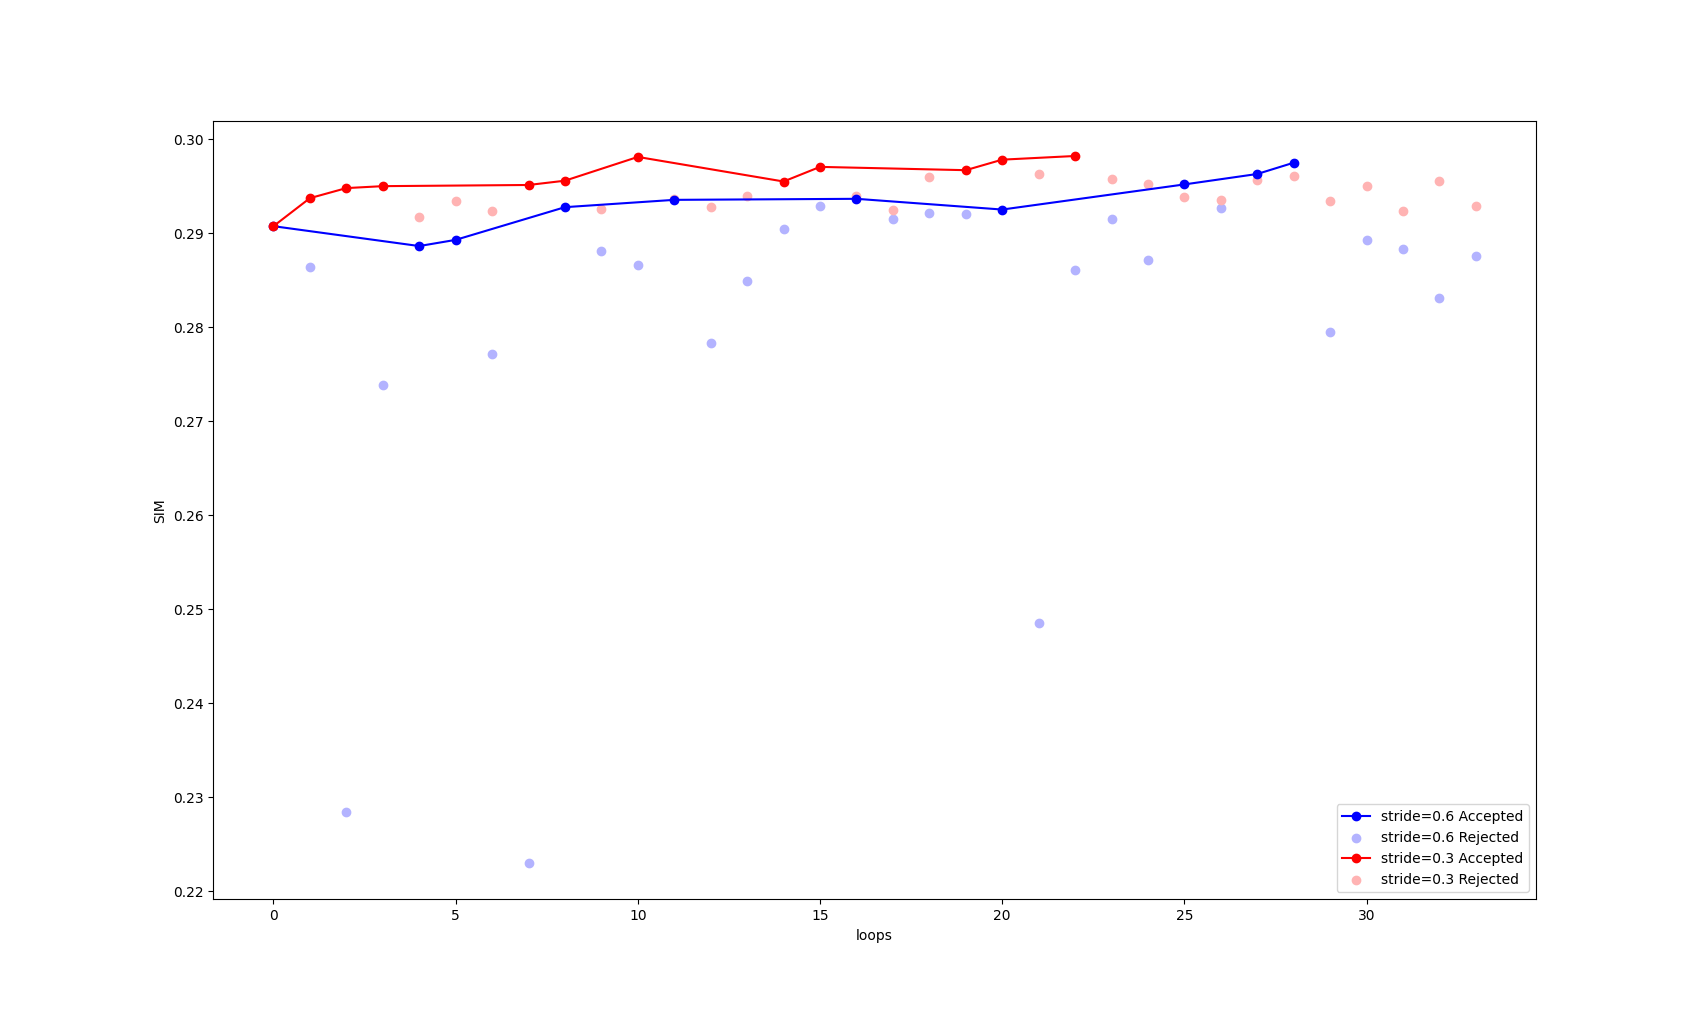
\includegraphics[width=10cm,height=7.5cm]{不同步长.png}
    \caption{SIM with Different Strides}
\end{figure}
\indent We can see that the group with a smaller step size reached the optimum value first and then remained relatively stable. On the other hand, the group with a larger step size took longer to reach the optimum value. The maximum SIM values obtained from the two groups with different step sizes are close, indicating that the model is not sensitive to this parameter.\\
\indent Next, we kept the initial values and strides of all parameters unchanged and only adjusted the initial and final temperatures of the algorithm to be (50,1) and (25,0.5) with a purpose of controlling the rounds. The results are as follows:
\begin{figure}[H]
    \centering
    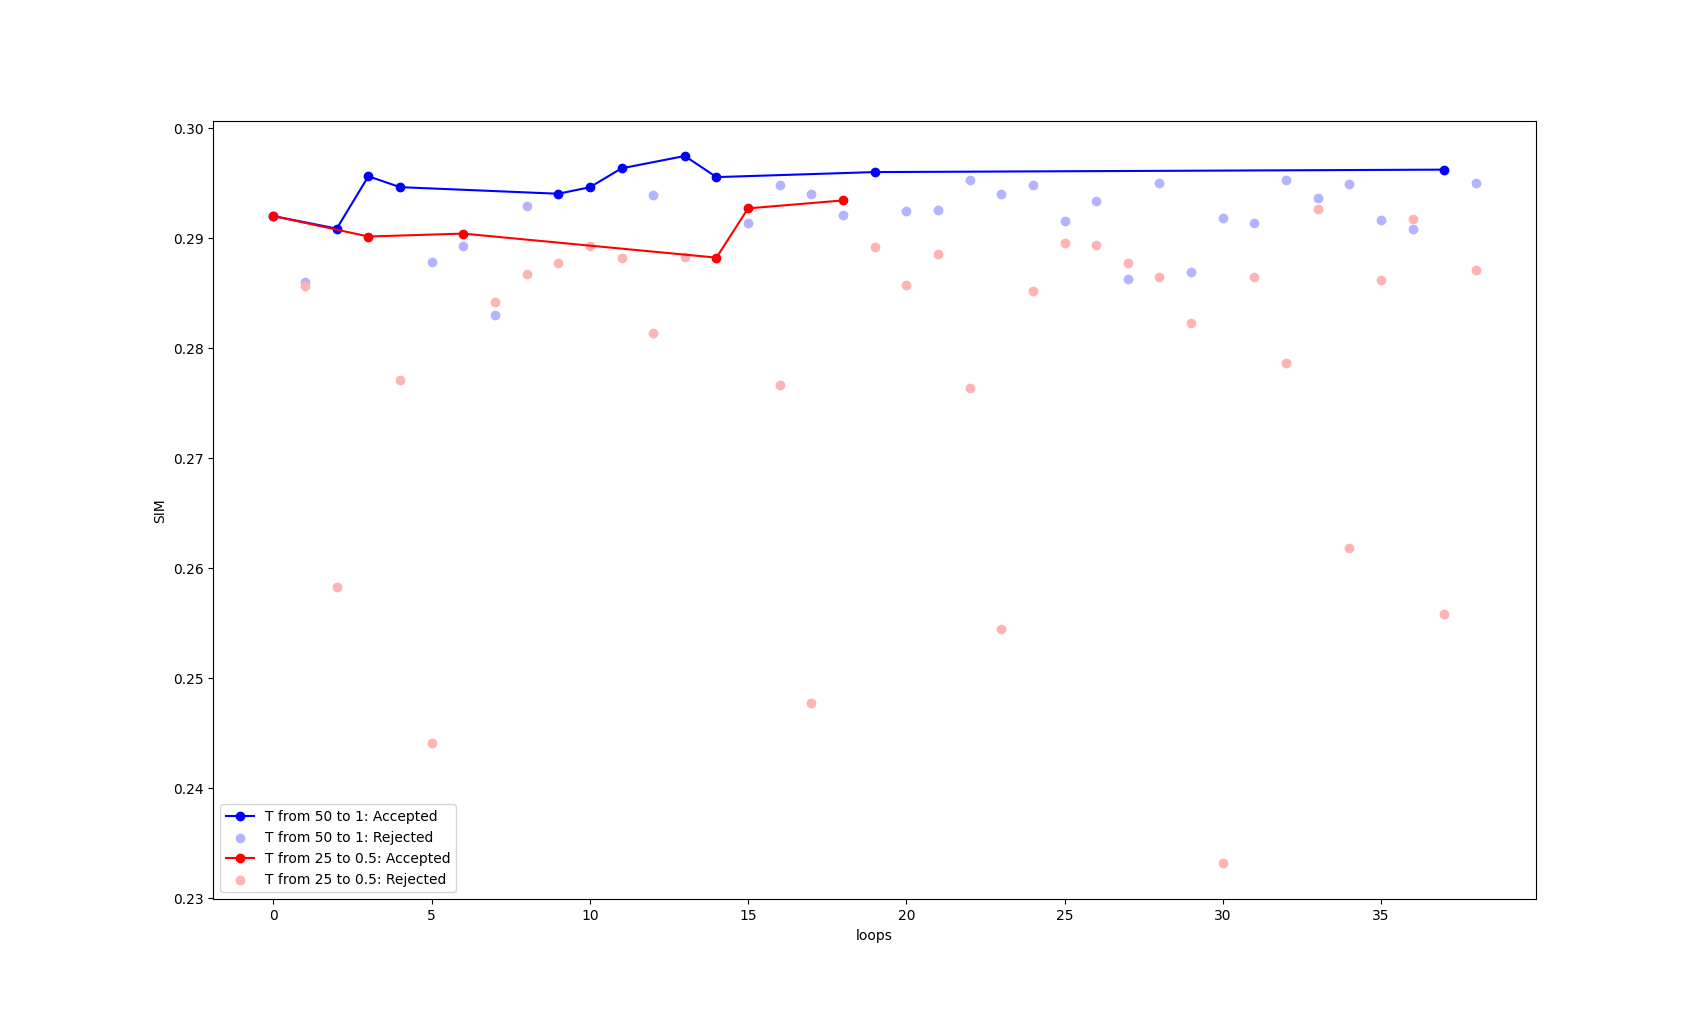
\includegraphics[width=8cm,height=6cm]{T.png}
    \caption{SIM with Different Initial and Final Temperatures}
\end{figure}
\indent We found that the group with a higher initial temperature calculated relatively higher results, while the group with a lower temperature had a lower probability of accepting smaller values, making it easier to reject smaller values and resulting in relatively lower results. However, there was no significant difference between the two groups, indicating a stable performance.\\
\indent To better showcase the tests we conducted, we have created the following table for comparison:
\begin{table}[H]%绘制结果权值表
    \begin{center}
        \caption{Robustness Test}{\vspace{0.5cm}}
        \begin{tabular}{cc}
        \hline
        \text{Trial}&\text{$SIM_{max}$}\\
        \hline
        \text{$T_0$=50  $T_{end}$=1 strides=0.3}&0.296183\\
        \hline
        \text{\quad $T_0$=25 $T_{end}$=0.5 strides=0.3}&0.293384\\       
        \hline
        \text{$T_0$=30  $T_{end}$=1 strides=0.6}&0.297507\\  
        \hline
        \text{$T_0$=30  $T_{end}$=1 strides=0.3}&0.298223\\       
        \hline
        \end{tabular}
    \end{center}
    \end{table}
\indent Considering the two indicators above, we believe that \textbf{our model exhibits strong stability and is not sensitive to changes in parameters}.

